% !TeX spellcheck = en_US

\chapter{Theoretical and Experimental Results}
\section{Training data}
\subsection{Airtiler - A data set generation tool}
For the training, we wanted to use publicly and freely available data. Not only due to the fact, highly resolved orthophotos cost quite a lot but also to make it possible for others to reproduce the results.

As a result of this, OpenStreetMap was chosen for the vector data and Microsoft Bing Maps for the imagery. A dataset consisting of satellite imagery and images for the ground truths can be created using the Python module Airtiler \cite{airtiler}. This tool has been developed by the author during this master thesis. It allows to configure one or more bounding boxes together with several other options like zoom level and OpenStreetMap attributes.

\autoref{lst:results:airtiler_config} shows a sample configuration as it is being used by Airtiler.

\begin{minipage}{\linewidth}
\begin{lstlisting}[caption={Sample configuration for Airtiler},captionpos=b,label=lst:results:airtiler_config]
{
  "options": {
    "target_dir": "",
    "zoom_levels": [18,19],
    "separate_instances": false
  },
  "query": {
    "tags": [
    	"highway",
    	"building",
    	"leisure=swimming_pool",
    	"sport=tennis",
    	"landuse=vineyard"
    ]
  },
  "boundingboxes": {
    "giswil_1": [
    	8.1566193073,
    	46.7783248574,
    	8.1681635349,
    	46.7905387509
    ],
    "giswil_2": [
    	8.1388001434,
    	46.7778439103,
    	8.1562840923,
    	46.7880064196
    ],
    "goldach_rorschacherberg": [
    	9.440673825,
    	47.4534664711,
    	9.5168056457,
    	47.4896115582
    ]
  }
}
\end{lstlisting}
\end{minipage}


In the next step, the configured bounding boxes are iterated and for each box all tiles, according to the Tile Map Service (TMS) specification \cite{tmsspec} are being processed. This includes the download of the corresponding orthophoto from Bing Maps, as well as the creation of at least one binary image, which contains all ground truth instances of the current class, for example \textit{building} or \textit{highway}, that have been specified in the configuration. As a result of this, one satellite image and one or more binary images are created per tile. If for the current tile no ground truths according to the configuration are found, no images for this tile will be created. \autoref{fig:results:airtiler_output_description} shows the output of a single tile, generated by Airtiler. One important point are the filenames, which are generated according to the content of the current file.

    \begin{figure}[H]
        \centering
        \begin{subfigure}[b]{0.475\textwidth}
            \centering
            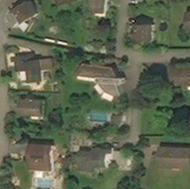
\includegraphics[width=\textwidth]{chapters/theoretical_and_experimental_results/images/18_138079_170377.png}
            \caption{\detokenize{18_138079_170377.tiff}}
            \label{fig:results:airtiler_output_orthophoto}
        \end{subfigure}
        \hfill
        \begin{subfigure}[b]{0.475\textwidth}  
            \centering 
            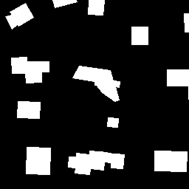
\includegraphics[width=\textwidth]{chapters/theoretical_and_experimental_results/images/18_138079_170377_building.png}
            \caption{\detokenize{18_138079_170377_building.tif}}
            \label{fig:results:airtiler_output_building}
        \end{subfigure}
        \vskip\baselineskip
        \begin{subfigure}[b]{0.475\textwidth}   
            \centering 
            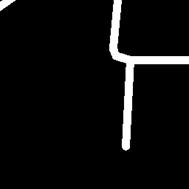
\includegraphics[width=\textwidth]{chapters/theoretical_and_experimental_results/images/18_138079_170377_highway.png}
            \caption{\detokenize{18_138079_170377_highway.tif}}
            \label{fig:results:airtiler_output_highway}
        \end{subfigure}
        \quad
        \begin{subfigure}[b]{0.475\textwidth}   
            \centering 
            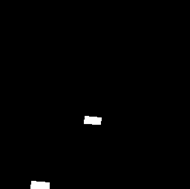
\includegraphics[width=\textwidth]{chapters/theoretical_and_experimental_results/images/18_138079_170377_swimming_pool.png}
            \caption{\detokenize{18_138079_170377_pool.tif}}
            \label{fig:results:airtiler_output_pool}
        \end{subfigure}
        \caption{Output of Airtiler for the TMS tile (x,y)=(138079,170377) at zoom level 18. The file names are generated according to the content, which makes the loading and interpretation of the data set rather simple; Images are named with the file extension \textit{.tiff} whereas the masks have the extension \textit{.tif}}
        \label{fig:results:airtiler_output_description}
    \end{figure}

\subsection{Publicly available data sets}
Furthermore, there are several different datasets publicly available: \cite{VolodymyrMnih.2013}, \cite{spacenet}, \cite{isprs-vaihingen}, \cite{isprs-potsdam}, \cite{Helber.20170831}, \cite{deepsat}.

\section{Mapping Challenge}
At the time of this writin the platform crowdAI hosted a challenge called Mapping Challenge \cite{mappingchallenge} which was about detecting buildings from satellite imagery. In order to gain additional knowledge regarding the performance of Mask R-CNN, we decided to participate in the challenge.

\autoref{tab:results:mapping_challenge_results} shows the changes made to the Mask R-CNN config and their impact on the prediction accuracy.

\newcolumntype{b}{>{\hsize=2.3\hsize}X}
\newcolumntype{s}{>{\hsize=.5\hsize}X}
\newcolumntype{m}{>{\hsize=.9\hsize}X}

\begin{table}[t]
\begin{tabularx}{\textwidth}{sssbss}
    \# Epochs & \# Steps / Epoch & \# Validation Steps & Config Change & AP@0.5 & AR@0.5 \\  \midrule
100 & 2500 & 150 & - & 0.798 & 0.566 \\ 
100 & 2500 & 150 & Image mean RGB updated & 0.799 & 0.564 \\ 
100 & 2500 & 150 & Mini mask disabled & 0.807 & 0.573 \\ 
100 & 5000 & 200 & + validation steps & 0.821 & 0.599 \\ 
100 & 10000 & 200 & + steps / epoch & 0.833 & 0.619 \\ 
100 & 20000 & 300 & + Validation steps, + steps / epoch & 0.853 & 0.885 \\  \bottomrule
\end{tabularx} 
    \caption{Mapping challenge results}
    \label{tab:results:mapping_challenge_results}
\end{table}

Generally, these results indicate, that finetuning of hyperparameters has an impact. Furthermore, the even bigger impact can be made just by longer training. However, in case of longer training, one has to make sure, that the network will not overfit. In the case of an already existing architecture like Mask R-CNN for example, this has already been done. On the other hand, if one develops a new architecture, overfitting has to be taken care of, for example with a technique called Dropout \cite{Srivastava.2014}. Generally, Dropout randomly disables some units during the training. As a result of this, the model constantly changes and overfitting can not happen that easily.

\section{Microsoft COCO Annotation Format}
For the crowdAI Mapping Challenge \cite{mappingchallenge} the instances were represented in the Microsoft COCO annotation format \cite{cocoformat}. Unfortunately, using this format, it is not possible to represent polygons with holes in it\footnote{\url{https://github.com/cocodataset/cocoapi/issues/153, 21.05.2018}}. As there are many buildings, for which this would be required, we decided not to use this format and instead use images for the representation of the ground truths.

\begin{figure}[H]
	\centering
	\begin{subfigure}{0.4\textwidth}
		\centering
    	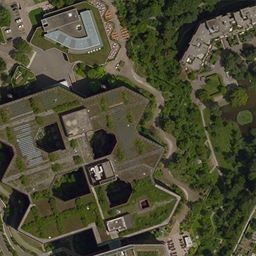
\includegraphics[width=0.9\linewidth]{chapters/theoretical_and_experimental_results/images/building_with_hole.png}		    \caption{A building with multiple holes}
	\end{subfigure}~
		\begin{subfigure}{0.4\textwidth}
		\centering
    	
\includegraphics[width=0.9\linewidth]{chapters/theoretical_and_experimental_results/images/building_with_hole_gt.png}		    \caption{Predicted building masks}
	\end{subfigure}
	\caption{The corresponding ground truth}
	\label{fig:results:buildings_with_holes_gt}
\end{figure}

\section{Building detection}
tbd